\chapter{Descripción de realización}

\section{Método de desarrollo}

Kingdom of Hatred se desarrollará mediante un sistema iterativo e incremental. Este proceso de desarrollo suple las carencias del modelo de cascada, el modelo tradicional que establece una rigorosa jerarquía en las fases del desarrollo y requiere completar una fase para comenzar la siguiente. En la Figura \ref{fig:modeloI} se puede observar el diagrama del modelo incremental.

\begin{figure}[!htp]
 \centering
 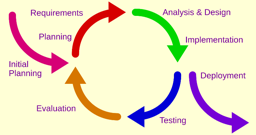
\includegraphics{fig/modelo_incremental}
 \caption{Modelo incremental}
 \label{fig:modeloI}
\end{figure}

El desarrollo incremental permite desarrollar una parte funcional del proyecto en cada etapa, reservando la mejora o extensión de funcionalidades para el futuro y por tanto controlando la complejidad y los riesgos. Además, este sistema permite a los desarrolladores aprovechar conocimiento adquirido en etapas previas e incorporar nuevo conocimiento y nuevas técnicas en fases venideras.

Adicionalmente, esta metodología confía en el desarrollo guiado por tests. Esta práctica consiste en el desarrollo de tests antes que código, y después se genera el mínimo código posible para completar esos tests. El objetivo de esta metodología es lograr código limpio y funcional, la idea es que los requisitos se traducen a evidencia, de forma que si los tests se completan satisfactoriamente, se garantiza que el software cubre dicho requisitos.

\subsection{Productos intermedios}

Los productos intermedios que se generarán en cada una de las fases son:

\begin{itemize}
	\item \textbf{Diseño del juego:}
	\begin{itemize}
		\item Documento de diseño de juego.
	\end{itemize}
	\item \textbf{Desarrollo del software:}
	\begin{itemize}
		\item Documento con la especificación del software.
	\end{itemize}
	\item \textbf{Validación técnica y usabilidad:}
	\begin{itemize}
		\item Informe de evaluación del juego.
	\end{itemize}
\end{itemize}

\subsection{EDT}

\begin{figure}[!htp]
	\centering
	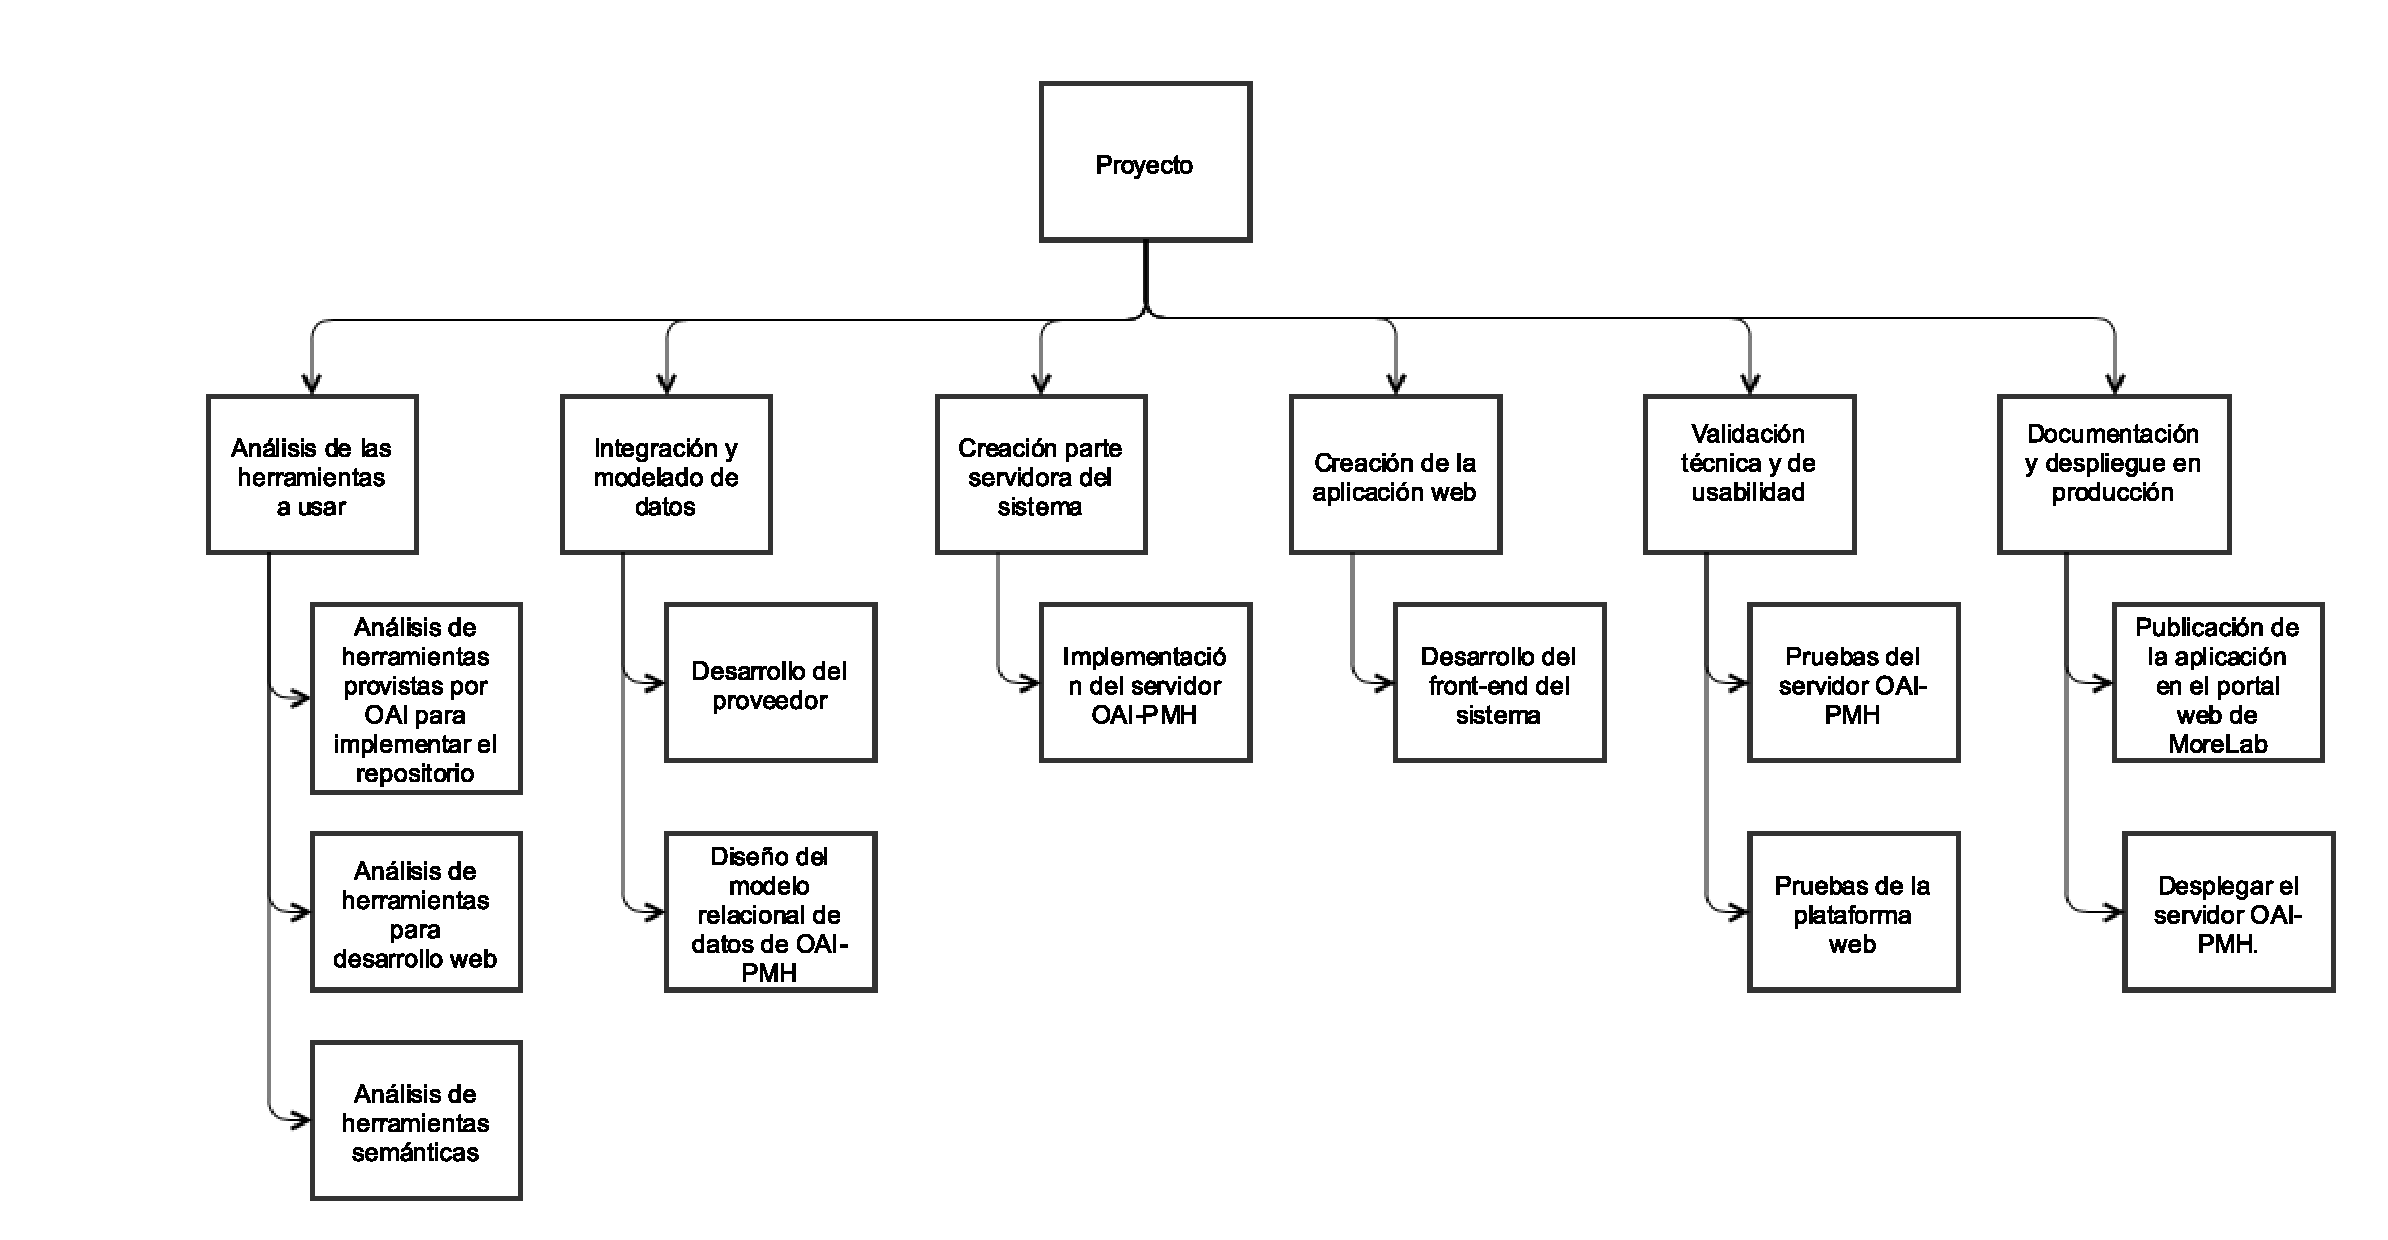
\includegraphics[angle=90, scale=.5]{fig/edt}
	\caption{EDT}
\end{figure}

\section{Tareas principales}

El desarrollo de Kingdom of Hatred comprende las siguientes tareas o actividades:

\subsection{Lanzamiento del proyecto}

\begin{itemize}
	\item \textbf{Organización}

	Actividad mediante la que se define y prepara la planificación, asignación de misiones y el lanzamiento del proyecto y sus sucesivas fases.
	\item \textbf{Seguimiento}

	Realización del seguimiento y control del desarrollo del proyecto, que permita la rápida detención y solución de problemas que puedan dificultar la buena marcha del mismo.
\end{itemize}

\subsection{Análisis de herramientas y técnicas}

\begin{itemize}
	\item \textbf{Análisis de herramientas para desarrollo de juegos}
	
	Investigar distintas alternativas que existen para el desarrollo de juegos.

	\item \textbf{Análisis de técnicas de generación procedural}
	Investigar distintos algoritmos de generación procedural que sean adecuados para la generación de niveles.
\end{itemize}

\subsection{Diseño del juego}

\begin{itemize}
	\item Diseño del juego
	Crear el documento de desarrollo de juego que definirá cómo será este.
\end{itemize}

\subsection{Desarrollo del software}

\begin{itemize}
	\item \textbf{Formación}
	Aprendizaje en la creación de juegos.
	\item \textbf{Diseño}
	Diseño del software del juego.
	\item \textbf{Implementación}
	Implementación del juego.
\end{itemize}

\subsection{Validación técnica y de usabilidad:}

\begin{itemize}
	\item \textbf{Betatesting}
	Uso intensivo del juego en busca de bugs.
	\item \textbf{Prueba de experiencia de usuario}
	Recoger opiniones para mejorar la experiencia de usuario.
\end{itemize}

\subsection{Distribución y cierre del proyecto}

\begin{itemize}
	\item \textbf{Despliegue de la versión final}
	
	Preparar el juego para el usuario final.
	\item \textbf{Cierre del proyecto}

	Cierre del proyecto.
\end{itemize}

\section{Hoja de Tareas}

% Tarea 1 %

\begin{center}
	\captionof{table}{Tareas 1-10}
	\begin{tabularx}{\textwidth}{@{\extracolsep{\fill} } | X | X | X |}
	\noalign{\hrule height 4pt}
	\multicolumn{3}{!{\vrule width 4pt} c !{\vrule width 4pt}}{\textbf{HOJA DE TAREAS}}	\\ \noalign{\hrule height 2pt}
	\multicolumn{3}{!{\vrule width 4pt} l !{\vrule width 4pt}}{\textbf{Nombre:} Unai Alonso Alvarez}	\\
	\multicolumn{3}{!{\vrule width 4pt} l !{\vrule width 4pt}}{\textbf{Fecha:} Marzo de 2015}			\\	\noalign{\hrule height 2pt}
	\multicolumn{2}{!{\vrule width 4pt} l}
	{
		\textbf{Identificación de Tarea:} T1-10
	}	&
		\multicolumn{1}{!{\vrule width 2pt} l !{\vrule width 4pt}}
		{
			\textbf{Duración:} 1 día
		}	\\	\Cline{2pt}{3-3}
	\multicolumn{2}{!{\vrule width 4pt} l}{\textbf{Descripción:}}	&
		\multicolumn{1}{!{\vrule width 2pt} l !{\vrule width 4pt}}
		{
			\textbf{Esfuerzo:} 3 horas
		}	\\
	\multicolumn{2}{!{\vrule width 4pt} p{0.7\linewidth}}
	{
		Seguimiento
	} &
		\multicolumn{1}{!{\vrule width 2pt} l !{\vrule width 4pt}}{}	\\	\noalign{\hrule height 2pt} 
	\multicolumn{2}{!{\vrule width 4pt} l}{\textbf{Criterios de Terminación:}}	&
		\multicolumn{1}{!{\vrule width 2pt} l !{\vrule width 4pt}}{\textbf{Tareas previas:}}	\\
	\multicolumn{2}{!{\vrule width 4pt} p{0.7\linewidth}}
	{
		Cuando el jefe de proyecto concluya que las tareas marchan adecuadamente respecto al plan de trabajo, o en caso contrario, cuando se haya definido y validado un plan de accion por el mismo jefe de proyecto.
	}	&
		\multicolumn{1}{!{\vrule width 2pt} l !{\vrule width 4pt}}
		{
			T11
		}	\\	\noalign{\hrule height 2pt}
	\multicolumn{2}{!{\vrule width 4pt} l}{\textbf{Competencias, conocimientos y notas:}} &
		\multicolumn{1}{!{\vrule width 2pt} l !{\vrule width 4pt}}{\textbf{Recursos:}}	\\
	\multicolumn{2}{!{\vrule width 4pt} p{0.7\linewidth}}
	{
		Persona encargada de dirigir el proyecto y con conocimiento de la marcha del proyecto.
	}	&
		\multicolumn{1}{!{\vrule width 2pt} p{0.2\textwidth} !{\vrule width 4pt}}
		{
			Jefe de proyecto
			
			Programador
		}	\\
	\noalign{\hrule height 4pt}
	\end{tabularx}
\end{center}

\clearpage

% Tarea 2 %

\begin{center}
	\captionof{table}{Tarea 11}
	\begin{tabularx}{\textwidth}{@{\extracolsep{\fill} } | X | X | X |}
	\noalign{\hrule height 4pt}
	\multicolumn{3}{!{\vrule width 4pt} c !{\vrule width 4pt}}{\textbf{HOJA DE TAREAS}}	\\ \noalign{\hrule height 2pt}
	\multicolumn{3}{!{\vrule width 4pt} l !{\vrule width 4pt}}{\textbf{Nombre:} Unai Alonso Alvarez}	\\
	\multicolumn{3}{!{\vrule width 4pt} l !{\vrule width 4pt}}{\textbf{Fecha:} Marzo de 2015}			\\	\noalign{\hrule height 2pt}
	\multicolumn{2}{!{\vrule width 4pt} l}
	{
		\textbf{Identificación de Tarea:} T11
	}	&
		\multicolumn{1}{!{\vrule width 2pt} l !{\vrule width 4pt}}
		{
			\textbf{Duración:} 2 días
		}	\\	\Cline{2pt}{3-3}
	\multicolumn{2}{!{\vrule width 4pt} l}{\textbf{Descripción:}}	&
		\multicolumn{1}{!{\vrule width 2pt} l !{\vrule width 4pt}}
		{
			\textbf{Esfuerzo:} 6 horas
		}	\\
	\multicolumn{2}{!{\vrule width 4pt} p{0.7\linewidth}}
	{
		Organización
	} &
		\multicolumn{1}{!{\vrule width 2pt} l !{\vrule width 4pt}}{}	\\	\noalign{\hrule height 2pt} 
	\multicolumn{2}{!{\vrule width 4pt} l}{\textbf{Criterios de Terminación:}}	&
		\multicolumn{1}{!{\vrule width 2pt} l !{\vrule width 4pt}}{\textbf{Tareas previas:}}	\\
	\multicolumn{2}{!{\vrule width 4pt} p{0.7\linewidth}}
	{
		Se ha definido la estrategia inicial para el desarrollo del proyecto y ha sido validada por el director del proyecto.
	}	&
		\multicolumn{1}{!{\vrule width 2pt} l !{\vrule width 4pt}}
		{
			Ninguna
		}	\\	\noalign{\hrule height 2pt}
	\multicolumn{2}{!{\vrule width 4pt} l}{\textbf{Competencias, conocimientos y notas:}} &
		\multicolumn{1}{!{\vrule width 2pt} l !{\vrule width 4pt}}{\textbf{Recursos:}}	\\
	\multicolumn{2}{!{\vrule width 4pt} p{0.7\linewidth}}
	{
		Persona encargada de dirigir el proyecto.
	}	&
		\multicolumn{1}{!{\vrule width 2pt} p{0.2\textwidth} !{\vrule width 4pt}}
		{
			Jefe de proyecto
		}	\\
	\noalign{\hrule height 4pt}
	\end{tabularx}
\end{center}

% Tarea 3 %

\begin{center}
	\captionof{table}{Tarea 12}
	\begin{tabularx}{\textwidth}{@{\extracolsep{\fill} } | X | X | X |}
	\noalign{\hrule height 4pt}
	\multicolumn{3}{!{\vrule width 4pt} c !{\vrule width 4pt}}{\textbf{HOJA DE TAREAS}}	\\ \noalign{\hrule height 2pt}
	\multicolumn{3}{!{\vrule width 4pt} l !{\vrule width 4pt}}{\textbf{Nombre:} Unai Alonso Alvarez}	\\
	\multicolumn{3}{!{\vrule width 4pt} l !{\vrule width 4pt}}{\textbf{Fecha:} Marzo de 2015}			\\	\noalign{\hrule height 2pt}
	\multicolumn{2}{!{\vrule width 4pt} l}
	{
		\textbf{Identificación de Tarea:} T12
	}	&
		\multicolumn{1}{!{\vrule width 2pt} l !{\vrule width 4pt}}
		{
			\textbf{Duración:} 3 días
		}	\\	\Cline{2pt}{3-3}
	\multicolumn{2}{!{\vrule width 4pt} l}{\textbf{Descripción:}}	&
		\multicolumn{1}{!{\vrule width 2pt} l !{\vrule width 4pt}}
		{
			\textbf{Esfuerzo:} 9 horas
		}	\\
	\multicolumn{2}{!{\vrule width 4pt} p{0.7\linewidth}}
	{
		Análisis de herramientas de desarrollo de juegos
	} &
		\multicolumn{1}{!{\vrule width 2pt} l !{\vrule width 4pt}}{}	\\	\noalign{\hrule height 2pt} 
	\multicolumn{2}{!{\vrule width 4pt} l}{\textbf{Criterios de Terminación:}}	&
		\multicolumn{1}{!{\vrule width 2pt} l !{\vrule width 4pt}}{\textbf{Tareas previas:}}	\\
	\multicolumn{2}{!{\vrule width 4pt} p{0.7\linewidth}}
	{
		 El programador ha decidido cuáles serán las herramientas a utilizar para el desarrollo del software en base a sus características y el jefe de proyecto ha validado que son adecuadas.
	}	&
		\multicolumn{1}{!{\vrule width 2pt} l !{\vrule width 4pt}}{T11}	\\	\noalign{\hrule height 2pt}
	\multicolumn{2}{!{\vrule width 4pt} l}{\textbf{Competencias, conocimientos y notas:}} &
		\multicolumn{1}{!{\vrule width 2pt} l !{\vrule width 4pt}}{\textbf{Recursos:}}	\\
	\multicolumn{2}{!{\vrule width 4pt} p{0.7\linewidth}}
	{
		Persona que se encargará de desarrollar el software.
	}	&
		\multicolumn{1}{!{\vrule width 2pt} p{0.2\textwidth} !{\vrule width 4pt}}
		{
			Ordenador

			Navegador de Internet

			Programador

		}	\\
	\noalign{\hrule height 4pt}
	\end{tabularx}
\end{center}

\clearpage

% Tarea 4 %

\begin{center}
	\captionof{table}{Tarea 13}
	\begin{tabularx}{\textwidth}{@{\extracolsep{\fill} } | X | X | X |}
	\noalign{\hrule height 4pt}
	\multicolumn{3}{!{\vrule width 4pt} c !{\vrule width 4pt}}{\textbf{HOJA DE TAREAS}}	\\ \noalign{\hrule height 2pt}
	\multicolumn{3}{!{\vrule width 4pt} l !{\vrule width 4pt}}{\textbf{Nombre:} Unai Alonso Alvarez}	\\
	\multicolumn{3}{!{\vrule width 4pt} l !{\vrule width 4pt}}{\textbf{Fecha:} Marzo de 2015}			\\	\noalign{\hrule height 2pt}
	\multicolumn{2}{!{\vrule width 4pt} l}
	{
		\textbf{Identificación de Tarea:} T13
	}	&
		\multicolumn{1}{!{\vrule width 2pt} l !{\vrule width 4pt}}
		{
			\textbf{Duración:} 3 días
		}	\\	\Cline{2pt}{3-3}
	\multicolumn{2}{!{\vrule width 4pt} l}{\textbf{Descripción:}}	&
		\multicolumn{1}{!{\vrule width 2pt} l !{\vrule width 4pt}}
		{
			\textbf{Esfuerzo:} 9 horas
		}	\\
	\multicolumn{2}{!{\vrule width 4pt} p{0.7\linewidth}}
	{
		 Análisis de algoritmos de generación procedural
	} &
		\multicolumn{1}{!{\vrule width 2pt} l !{\vrule width 4pt}}{}	\\	\noalign{\hrule height 2pt} 
	\multicolumn{2}{!{\vrule width 4pt} l}{\textbf{Criterios de Terminación:}}	&
		\multicolumn{1}{!{\vrule width 2pt} l !{\vrule width 4pt}}{\textbf{Tareas previas:}}	\\
	\multicolumn{2}{!{\vrule width 4pt} p{0.7\linewidth}}
	{
		El programador ha decidido cuáles serán los algoritmos a utilizar para la generación aleatoria de escenarios y el jefe de proyecto ha validado que son adecuadas.
	}	&
		\multicolumn{1}{!{\vrule width 2pt} l !{\vrule width 4pt}}{T12}	\\	\noalign{\hrule height 2pt}
	\multicolumn{2}{!{\vrule width 4pt} l}{\textbf{Competencias, conocimientos y notas:}} &
		\multicolumn{1}{!{\vrule width 2pt} l !{\vrule width 4pt}}{\textbf{Recursos:}}	\\
	\multicolumn{2}{!{\vrule width 4pt} p{0.7\linewidth}}
	{
		Persona que se encargará de implementar los algoritmos.
	}	&
		\multicolumn{1}{!{\vrule width 2pt} p{0.2\textwidth} !{\vrule width 4pt}}
		{
			Ordenador

			Navegador de internet

			Programador

		}	\\
	\noalign{\hrule height 4pt}
	\end{tabularx}
\end{center}

% Tarea 5 %

\begin{center}
	\captionof{table}{Tarea 14}
	\begin{tabularx}{\textwidth}{@{\extracolsep{\fill} } | X | X | X |}
	\noalign{\hrule height 4pt}
	\multicolumn{3}{!{\vrule width 4pt} c !{\vrule width 4pt}}{\textbf{HOJA DE TAREAS}}	\\ \noalign{\hrule height 2pt}
	\multicolumn{3}{!{\vrule width 4pt} l !{\vrule width 4pt}}{\textbf{Nombre:} Unai Alonso Alvarez}	\\
	\multicolumn{3}{!{\vrule width 4pt} l !{\vrule width 4pt}}{\textbf{Fecha:} Marzo de 2015}			\\	\noalign{\hrule height 2pt}
	\multicolumn{2}{!{\vrule width 4pt} l}
	{
		\textbf{Identificación de Tarea:} T14
	}	&
		\multicolumn{1}{!{\vrule width 2pt} l !{\vrule width 4pt}}
		{
			\textbf{Duración:} 5 días
		}	\\	\Cline{2pt}{3-3}
	\multicolumn{2}{!{\vrule width 4pt} l}{\textbf{Descripción:}}	&
		\multicolumn{1}{!{\vrule width 2pt} l !{\vrule width 4pt}}
		{
			\textbf{Esfuerzo:} 15 horas
		}	\\
	\multicolumn{2}{!{\vrule width 4pt} p{0.7\linewidth}}
	{
		Diseño del juego
	} &
		\multicolumn{1}{!{\vrule width 2pt} l !{\vrule width 4pt}}{}	\\	\noalign{\hrule height 2pt} 
	\multicolumn{2}{!{\vrule width 4pt} l}{\textbf{Criterios de Terminación:}}	&
		\multicolumn{1}{!{\vrule width 2pt} l !{\vrule width 4pt}}{\textbf{Tareas previas:}}	\\
	\multicolumn{2}{!{\vrule width 4pt} p{0.7\linewidth}}
	{
		Se ha producido un documento de diseño de juego completo y el director del proyecto lo aprueba.
	}	&
		\multicolumn{1}{!{\vrule width 2pt} l !{\vrule width 4pt}}{T11}	\\	\noalign{\hrule height 2pt}
	\multicolumn{2}{!{\vrule width 4pt} l}{\textbf{Competencias, conocimientos y notas:}} &
		\multicolumn{1}{!{\vrule width 2pt} l !{\vrule width 4pt}}{\textbf{Recursos:}}	\\
	\multicolumn{2}{!{\vrule width 4pt} p{0.7\linewidth}}
	{
		Persona encargada de diseñar el juego y dirigir su creación.
	}	&
		\multicolumn{1}{!{\vrule width 2pt} p{0.2\textwidth} !{\vrule width 4pt}}
		{
			Ordenador

			Jefe de proyecto
		}	\\
	\noalign{\hrule height 4pt}
	\end{tabularx}
\end{center}

% Tarea 6 %

\begin{center}
	\captionof{table}{Tarea 15}
	\begin{tabularx}{\textwidth}{@{\extracolsep{\fill} } | X | X | X |}
	\noalign{\hrule height 4pt}
	\multicolumn{3}{!{\vrule width 4pt} c !{\vrule width 4pt}}{\textbf{HOJA DE TAREAS}}	\\ \noalign{\hrule height 2pt}
	\multicolumn{3}{!{\vrule width 4pt} l !{\vrule width 4pt}}{\textbf{Nombre:} Unai Alonso Alvarez}	\\
	\multicolumn{3}{!{\vrule width 4pt} l !{\vrule width 4pt}}{\textbf{Fecha:} Marzo de 2015}			\\	\noalign{\hrule height 2pt}
	\multicolumn{2}{!{\vrule width 4pt} l}
	{
		\textbf{Identificación de Tarea:} T15
	}	&
		\multicolumn{1}{!{\vrule width 2pt} l !{\vrule width 4pt}}
		{
			\textbf{Duración:} 15 días
		}	\\	\Cline{2pt}{3-3}
	\multicolumn{2}{!{\vrule width 4pt} l}{\textbf{Descripción:}}	&
		\multicolumn{1}{!{\vrule width 2pt} l !{\vrule width 4pt}}
		{
			\textbf{Esfuerzo:} 45 horas
		}	\\
	\multicolumn{2}{!{\vrule width 4pt} p{0.7\linewidth}}
	{
		Formación
	} &
		\multicolumn{1}{!{\vrule width 2pt} l !{\vrule width 4pt}}{}	\\	\noalign{\hrule height 2pt} 
	\multicolumn{2}{!{\vrule width 4pt} l}{\textbf{Criterios de Terminación:}}	&
		\multicolumn{1}{!{\vrule width 2pt} l !{\vrule width 4pt}}{\textbf{Tareas previas:}}	\\
	\multicolumn{2}{!{\vrule width 4pt} p{0.7\linewidth}}
	{
		El programador conoce y es capaz de desenvolverse con las herramientas a utilizar.
	}	&
		\multicolumn{1}{!{\vrule width 2pt} l !{\vrule width 4pt}}
		{
			T13
		}	\\	\noalign{\hrule height 2pt}
	\multicolumn{2}{!{\vrule width 4pt} l}{\textbf{Competencias, conocimientos y notas:}} &
		\multicolumn{1}{!{\vrule width 2pt} l !{\vrule width 4pt}}{\textbf{Recursos:}}	\\
	\multicolumn{2}{!{\vrule width 4pt} p{0.7\linewidth}}
	{
		Persona encargada de implementar el juego.
	}	&
		\multicolumn{1}{!{\vrule width 2pt} l !{\vrule width 4pt}}{\parbox{0.2\textwidth}
		{
			Ordenador

			Programador
		}}	\\
	\noalign{\hrule height 4pt}
	\end{tabularx}
\end{center}

% Tarea 7 %

\begin{center}
	\captionof{table}{Tarea 16}
	\begin{tabularx}{\textwidth}{@{\extracolsep{\fill} } | X | X | X |}
	\noalign{\hrule height 4pt}
	\multicolumn{3}{!{\vrule width 4pt} c !{\vrule width 4pt}}{\textbf{HOJA DE TAREAS}}	\\ \noalign{\hrule height 2pt}
	\multicolumn{3}{!{\vrule width 4pt} l !{\vrule width 4pt}}{\textbf{Nombre:} Unai Alonso Alvarez}	\\
	\multicolumn{3}{!{\vrule width 4pt} l !{\vrule width 4pt}}{\textbf{Fecha:} Marzo de 2015}			\\	\noalign{\hrule height 2pt}
	\multicolumn{2}{!{\vrule width 4pt} l}
	{
		\textbf{Identificación de Tarea:} T16
	}	&
		\multicolumn{1}{!{\vrule width 2pt} l !{\vrule width 4pt}}
		{
			\textbf{Duración:} 15 días
		}	\\	\Cline{2pt}{3-3}
	\multicolumn{2}{!{\vrule width 4pt} l}{\textbf{Descripción:}}	&
		\multicolumn{1}{!{\vrule width 2pt} l !{\vrule width 4pt}}
		{
			\textbf{Esfuerzo:} 45 horas
		}	\\
	\multicolumn{2}{!{\vrule width 4pt} p{0.7\linewidth}}
	{
		Diseño del software.
	} &
		\multicolumn{1}{!{\vrule width 2pt} l !{\vrule width 4pt}}{}	\\	\noalign{\hrule height 2pt} 
	\multicolumn{2}{!{\vrule width 4pt} l}{\textbf{Criterios de Terminación:}}	&
		\multicolumn{1}{!{\vrule width 2pt} l !{\vrule width 4pt}}{\textbf{Tareas previas:}}	\\
	\multicolumn{2}{!{\vrule width 4pt} p{0.7\linewidth}}
	{
		Se ha generado un documento detallando el diseño del software y el director de proyecto lo aprueba.
	}	&
		\multicolumn{1}{!{\vrule width 2pt} l !{\vrule width 4pt}}
		{
			T14
			T15
		}	\\	\noalign{\hrule height 2pt}
	\multicolumn{2}{!{\vrule width 4pt} l}{\textbf{Competencias, conocimientos y notas:}} &
		\multicolumn{1}{!{\vrule width 2pt} l !{\vrule width 4pt}}{\textbf{Recursos:}}	\\
	\multicolumn{2}{!{\vrule width 4pt} p{0.7\linewidth}}
	{
		Persona encargada de implementar el juego.

	}	&
		\multicolumn{1}{!{\vrule width 2pt} l !{\vrule width 4pt}}{\parbox{0.2\textwidth}
		{
			Programador

			Ordenador
		}}	\\
	\noalign{\hrule height 4pt}
	\end{tabularx}
\end{center}

% tarea 8 %

\begin{center}
	\captionof{table}{Tarea 17}
	\begin{tabularx}{\textwidth}{@{\extracolsep{\fill} } | X | X | X |}
	\noalign{\hrule height 4pt}
	\multicolumn{3}{!{\vrule width 4pt} c !{\vrule width 4pt}}{\textbf{HOJA DE TAREAS}}	\\ \noalign{\hrule height 2pt}
	\multicolumn{3}{!{\vrule width 4pt} l !{\vrule width 4pt}}{\textbf{Nombre:} Unai Alonso Alvarez}	\\
	\multicolumn{3}{!{\vrule width 4pt} l !{\vrule width 4pt}}{\textbf{Fecha:} Marzo de 2015}			\\	\noalign{\hrule height 2pt}
	\multicolumn{2}{!{\vrule width 4pt} l}
	{
		\textbf{Identificación de Tarea:} T17
	}	&
		\multicolumn{1}{!{\vrule width 2pt} l !{\vrule width 4pt}}
		{
			\textbf{Duración:} 30 días
		}	\\	\Cline{2pt}{3-3}
	\multicolumn{2}{!{\vrule width 4pt} l}{\textbf{Descripción:}}	&
		\multicolumn{1}{!{\vrule width 2pt} l !{\vrule width 4pt}}
		{
			\textbf{Esfuerzo:} 90 horas
		}	\\
	\multicolumn{2}{!{\vrule width 4pt} p{0.7\linewidth}}
	{
		Implementación
	} &
		\multicolumn{1}{!{\vrule width 2pt} l !{\vrule width 4pt}}{}	\\	\noalign{\hrule height 2pt} 
	\multicolumn{2}{!{\vrule width 4pt} l}{\textbf{Criterios de Terminación:}}	&
		\multicolumn{1}{!{\vrule width 2pt} l !{\vrule width 4pt}}{\textbf{Tareas previas:}}	\\
	\multicolumn{2}{!{\vrule width 4pt} p{0.7\linewidth}}
	{
		Se ha generado una versión de software con todas las funcionalidades implementadas y el director lo aprueba.
	}	&
		\multicolumn{1}{!{\vrule width 2pt} l !{\vrule width 4pt}}
		{
			T16
		}	\\	\noalign{\hrule height 2pt}
	\multicolumn{2}{!{\vrule width 4pt} l}{\textbf{Competencias, conocimientos y notas:}} &
		\multicolumn{1}{!{\vrule width 2pt} l !{\vrule width 4pt}}{\textbf{Recursos:}}	\\
	\multicolumn{2}{!{\vrule width 4pt} p{0.7\linewidth}}
	{
		Persona encargada de implementar el juego.
	}	&
		\multicolumn{1}{!{\vrule width 2pt} l !{\vrule width 4pt}}{\parbox{0.2\textwidth}
		{
			Programador

			Ordenador
		}}	\\
	\noalign{\hrule height 4pt}
	\end{tabularx}
\end{center}

% Tarea 9 %

\begin{center}
	\captionof{table}{Tarea 18}
	\begin{tabularx}{\textwidth}{@{\extracolsep{\fill} } | X | X | X |}
	\noalign{\hrule height 4pt}
	\multicolumn{3}{!{\vrule width 4pt} c !{\vrule width 4pt}}{\textbf{HOJA DE TAREAS}}	\\ \noalign{\hrule height 2pt}
	\multicolumn{3}{!{\vrule width 4pt} l !{\vrule width 4pt}}{\textbf{Nombre:} Unai Alonso Alvarez}	\\
	\multicolumn{3}{!{\vrule width 4pt} l !{\vrule width 4pt}}{\textbf{Fecha:} Marzo de 2015}			\\	\noalign{\hrule height 2pt}
	\multicolumn{2}{!{\vrule width 4pt} l}
	{
		\textbf{Identificación de Tarea:} T18
	}	&
		\multicolumn{1}{!{\vrule width 2pt} l !{\vrule width 4pt}}
		{
			\textbf{Duración:} 15 días
		}	\\	\Cline{2pt}{3-3}
	\multicolumn{2}{!{\vrule width 4pt} l}{\textbf{Descripción:}}	&
		\multicolumn{1}{!{\vrule width 2pt} l !{\vrule width 4pt}}
		{
			\textbf{Esfuerzo:} 45 horas
		}	\\
	\multicolumn{2}{!{\vrule width 4pt} p{0.7\linewidth}}
	{
		Betatesting
	} &
		\multicolumn{1}{!{\vrule width 2pt} l !{\vrule width 4pt}}{}	\\	\noalign{\hrule height 2pt} 
	\multicolumn{2}{!{\vrule width 4pt} l}{\textbf{Criterios de Terminación:}}	&
		\multicolumn{1}{!{\vrule width 2pt} l !{\vrule width 4pt}}{\textbf{Tareas previas:}}	\\
	\multicolumn{2}{!{\vrule width 4pt} p{0.7\linewidth}}
	{
		El jefe de proyecto acepta el estado actual del juego como válido o se termina el tiempo asignado a la tarea
	}	&
		\multicolumn{1}{!{\vrule width 2pt} l !{\vrule width 4pt}}
		{
			T17
		}	\\	\noalign{\hrule height 2pt}
	\multicolumn{2}{!{\vrule width 4pt} l}{\textbf{Competencias, conocimientos y notas:}} &
		\multicolumn{1}{!{\vrule width 2pt} l !{\vrule width 4pt}}{\textbf{Recursos:}}	\\
	\multicolumn{2}{!{\vrule width 4pt} p{0.7\linewidth}}
	{
		Persona encargada de implementar el juego, que corregira los errores que se encuentren.

		Persona encargada de probar intensivamente el software en busca de errores.
	}	&
		\multicolumn{1}{!{\vrule width 2pt} l !{\vrule width 4pt}}{\parbox{0.2\textwidth}
		{
			Programador

			Tester

			Ordenador

			Juego
		}}	\\
	\noalign{\hrule height 4pt}
	\end{tabularx}
\end{center}

\clearpage

% Tarea 10 %

\begin{center}
	\captionof{table}{Tarea 19}
	\begin{tabularx}{\textwidth}{@{\extracolsep{\fill} } | X | X | X |}
	\noalign{\hrule height 4pt}
	\multicolumn{3}{!{\vrule width 4pt} c !{\vrule width 4pt}}{\textbf{HOJA DE TAREAS}}	\\ \noalign{\hrule height 2pt}
	\multicolumn{3}{!{\vrule width 4pt} l !{\vrule width 4pt}}{\textbf{Nombre:} Unai Alonso Alvarez}	\\
	\multicolumn{3}{!{\vrule width 4pt} l !{\vrule width 4pt}}{\textbf{Fecha:} Marzo de 2015}			\\	\noalign{\hrule height 2pt}
	\multicolumn{2}{!{\vrule width 4pt} l}
	{
		\textbf{Identificación de Tarea:} T19
	}	&
		\multicolumn{1}{!{\vrule width 2pt} l !{\vrule width 4pt}}
		{
			\textbf{Duración:} 15 días
		}	\\	\Cline{2pt}{3-3}
	\multicolumn{2}{!{\vrule width 4pt} l}{\textbf{Descripción:}}	&
		\multicolumn{1}{!{\vrule width 2pt} l !{\vrule width 4pt}}
		{
			\textbf{Esfuerzo:} 45 horas
		}	\\
	\multicolumn{2}{!{\vrule width 4pt} p{0.7\linewidth}}
	{
		Prueba de experiencia de usuario
	} &
		\multicolumn{1}{!{\vrule width 2pt} l !{\vrule width 4pt}}{}	\\	\noalign{\hrule height 2pt} 
	\multicolumn{2}{!{\vrule width 4pt} l}{\textbf{Criterios de Terminación:}}	&
		\multicolumn{1}{!{\vrule width 2pt} l !{\vrule width 4pt}}{\textbf{Tareas previas:}}	\\
	\multicolumn{2}{!{\vrule width 4pt} p{0.7\linewidth}}
	{
		El jefe de proyecto acepta la experiencia actual como válida o se ha terminado el tiempo asignado para la tarea.
	}	&
		\multicolumn{1}{!{\vrule width 2pt} l !{\vrule width 4pt}}
		{
			T18
		}	\\	\noalign{\hrule height 2pt}
	\multicolumn{2}{!{\vrule width 4pt} l}{\textbf{Competencias, conocimientos y notas:}} &
		\multicolumn{1}{!{\vrule width 2pt} l !{\vrule width 4pt}}{\textbf{Recursos:}}	\\
	\multicolumn{2}{!{\vrule width 4pt} p{0.7\linewidth}}
	{
		Persona encargada de implementar el juego, que modificara lo que sea necesario.

		Personas encargadas de probar el software y definir su usabilidad.
	}	&
		\multicolumn{1}{!{\vrule width 2pt} l !{\vrule width 4pt}}{\parbox{0.2\textwidth}
		{
			Programador

			Tester

			Ordenador

			Juego
		}}	\\
	\noalign{\hrule height 4pt}
	\end{tabularx}
\end{center}

% Tarea 11 %

\begin{center}
	\captionof{table}{Tarea 20}
	\begin{tabularx}{\textwidth}{@{\extracolsep{\fill} } | X | X | X |}
	\noalign{\hrule height 4pt}
	\multicolumn{3}{!{\vrule width 4pt} c !{\vrule width 4pt}}{\textbf{HOJA DE TAREAS}}	\\ \noalign{\hrule height 2pt}
	\multicolumn{3}{!{\vrule width 4pt} l !{\vrule width 4pt}}{\textbf{Nombre:} Unai Alonso Alvarez}	\\
	\multicolumn{3}{!{\vrule width 4pt} l !{\vrule width 4pt}}{\textbf{Fecha:} Marzo de 2015}			\\	\noalign{\hrule height 2pt}
	\multicolumn{2}{!{\vrule width 4pt} l}
	{
		\textbf{Identificación de Tarea:} T20
	}	&
		\multicolumn{1}{!{\vrule width 2pt} l !{\vrule width 4pt}}
		{
			\textbf{Duración:} 5 días
		}	\\	\Cline{2pt}{3-3}
	\multicolumn{2}{!{\vrule width 4pt} l}{\textbf{Descripción:}}	&
		\multicolumn{1}{!{\vrule width 2pt} l !{\vrule width 4pt}}
		{
			\textbf{Esfuerzo:} 15 horas
		}	\\
	\multicolumn{2}{!{\vrule width 4pt} p{0.7\linewidth}}
	{
		Despliegue de la versión final
	} &
		\multicolumn{1}{!{\vrule width 2pt} l !{\vrule width 4pt}}{}	\\	\noalign{\hrule height 2pt} 
	\multicolumn{2}{!{\vrule width 4pt} l}{\textbf{Criterios de Terminación:}}	&
		\multicolumn{1}{!{\vrule width 2pt} l !{\vrule width 4pt}}{\textbf{Tareas previas:}}	\\
	\multicolumn{2}{!{\vrule width 4pt} p{0.7\linewidth}}
	{
		Se ha generado un ejecutable que funcionará en cualquier ordenador de las plataformas destinadas.
	}	&
		\multicolumn{1}{!{\vrule width 2pt} l !{\vrule width 4pt}}
		{
			T19
		}	\\	\noalign{\hrule height 2pt}
	\multicolumn{2}{!{\vrule width 4pt} l}{\textbf{Competencias, conocimientos y notas:}} &
		\multicolumn{1}{!{\vrule width 2pt} l !{\vrule width 4pt}}{\textbf{Recursos:}}	\\
	\multicolumn{2}{!{\vrule width 4pt} p{0.7\linewidth}}
	{
		Persona encargada de implementar el juego, que generará la versión final.
	}	&
		\multicolumn{1}{!{\vrule width 2pt} l !{\vrule width 4pt}}{\parbox{0.2\textwidth}
		{
			Programador

			Ordenador

			Juego
		}}	\\
	\noalign{\hrule height 4pt}
	\end{tabularx}
\end{center}

% Tarea 12 %

\begin{center}
	\captionof{table}{Tarea 21}
	\begin{tabularx}{\textwidth}{@{\extracolsep{\fill} } | X | X | X |}
	\noalign{\hrule height 4pt}
	\multicolumn{3}{!{\vrule width 4pt} c !{\vrule width 4pt}}{\textbf{HOJA DE TAREAS}}	\\ \noalign{\hrule height 2pt}
	\multicolumn{3}{!{\vrule width 4pt} l !{\vrule width 4pt}}{\textbf{Nombre:} Unai Alonso Alvarez}	\\
	\multicolumn{3}{!{\vrule width 4pt} l !{\vrule width 4pt}}{\textbf{Fecha:} Marzo de 2015}			\\	\noalign{\hrule height 2pt}
	\multicolumn{2}{!{\vrule width 4pt} l}
	{
		\textbf{Identificación de Tarea:} T21
	}	&
		\multicolumn{1}{!{\vrule width 2pt} l !{\vrule width 4pt}}
		{
			\textbf{Duración:} 1 día
		}	\\	\Cline{2pt}{3-3}
	\multicolumn{2}{!{\vrule width 4pt} l}{\textbf{Descripción:}}	&
		\multicolumn{1}{!{\vrule width 2pt} l !{\vrule width 4pt}}
		{
			\textbf{Esfuerzo:} 3 horas
		}	\\
	\multicolumn{2}{!{\vrule width 4pt} p{0.7\linewidth}}
	{
		Cierre del proyecto
	} &
		\multicolumn{1}{!{\vrule width 2pt} l !{\vrule width 4pt}}{}	\\	\noalign{\hrule height 2pt} 
	\multicolumn{2}{!{\vrule width 4pt} l}{\textbf{Criterios de Terminación:}}	&
		\multicolumn{1}{!{\vrule width 2pt} l !{\vrule width 4pt}}{\textbf{Tareas previas:}}	\\
	\multicolumn{2}{!{\vrule width 4pt} p{0.7\linewidth}}
	{
		Todas las tareas del proyecto han sido terminadas y se ha aprendido de la experiencia.
	}	&
		\multicolumn{1}{!{\vrule width 2pt} l !{\vrule width 4pt}}
		{
			T10, T20
		}	\\	\noalign{\hrule height 2pt}
	\multicolumn{2}{!{\vrule width 4pt} l}{\textbf{Competencias, conocimientos y notas:}} &
		\multicolumn{1}{!{\vrule width 2pt} l !{\vrule width 4pt}}{\textbf{Recursos:}}	\\
	\multicolumn{2}{!{\vrule width 4pt} p{0.7\linewidth}}
	{
		Programador, que aportará su experiencia.

		Jefe de proyecto, que se encargará de la gestión del conocimiento.
	}	&
		\multicolumn{1}{!{\vrule width 2pt} l !{\vrule width 4pt}}{\parbox{0.2\textwidth}
		{
			Programador

			Ordenador

			Jefe de proyecto
		}}	\\
	\noalign{\hrule height 4pt}
	\end{tabularx}
\end{center}

\chapter{Organización, Equipo}

\section{Esquema organizativo}

La organización del proyecto se articula en torno al comité de dirección y al equipo de trabajo que se va a encargar de desarrollar el producto, en función de la estructura de la Figura \ref{fig:esqOrg}.

\begin{figure}[!htp]
	\centering
	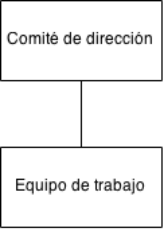
\includegraphics[scale=.75]{fig/esq}
	\caption{Esquema Organizativo}
	\label{fig:esqOrg}
\end{figure}

\begin{itemize}
	\item Comité de dirección 
	Su función principal es asesorar el proyecto y la toma de decisiones. Formado por el jefe de proyecto.
	\item Equipo de trabajo
	El órgano encargado de diseñar, desarrollar y testear el contenido del proyecto en función de las diferentes fases estipuladas. Formado por el programador, el diseñador y el tester.
\end{itemize}

\section{Plan de Recursos Humanos}
\label{sec:planRecursosHumanos}

El equipo de trabajo estará formado por los siguientes perfiles directamente relacionados con las diferentes áreas de competencias que abordan el proyecto:

\begin{itemize}
	\item Jefe de proyecto:
	Sus funciones son realizar las actividades de organización, coordinación y seguimiento del proyecto. Por otro lado, deberá encargarse del diseño del juego. Con un jefe de proyecto es suficiente. Para el perfil será necesario alguien con experiencia en comunicación interpersonal, liderazgo y solución de problemas.
	\item Programador:
	Encargado de diseñar e implementar el software en base al diseño del 	juego. Será necesario conocimiento de ingeniería del software para llevar a cabo las tareas asignadas a este perfil.
	\item Tester:
	Encargado de probar el producto y reportar errores y sugerir mejoras. 	Para hacer las 	pruebas de fase beta será suficiente con un tester. 	Sin embargo, para las prueba de 	experiencia de usuario sería 	conveniente contar con el mayor número de personas 	posibles. El tester debe ser tener imaginación y ser creativo para llevar al juego a situaciones límite y encontrar el mayor número de errores posible.
\end{itemize}

\chapter{Condiciones de ejecución}

\section{Entorno de trabajo}

El lugar de trabajo habitual será el domicilio del trabajador.
El calendario y horario serán 3 horas al día, preferiblemente de lunes a viernes.
Los medios informáticos para la ejecución corren a cargo del trabajador. Los medios de los que se disponen actualmente y se usarán son los siguientes: 

\begin{itemize}
	\item Hardware
	\begin{itemize}
		\item Ordenador de sobremesa completo con monitor secundario
		\item Ordenador portátil
	\end{itemize}
	\item Software
	\begin{itemize}
		\item Todo el software que se use será gratuito, así que este apartado no supondrá un problema.
	\end{itemize}
\end{itemize}

\section{Control de cambios}

Tanto jefe de proyecto como el tutor tienen potestad para pedir modificaciones en las 	especificaciones, diseños o desarrollos ya realizados. En caso de querer modificar algo, se 	seguirá el siguiente procedimiento:

\begin{enumerate}
	\item Comunicación formal del solicitante de las modificaciones solicitadas.
	\item Valoración, por parte del jefe del proyecto y el equipo de desarrollo, de la repercusión 	técnica, económica y el plazo de ejecución.
	\item Presentación de una propuesta valorada al solicitante.
	\item Notificación, por parte del solicitante, de la aprobación o no de la propuesta.
	\item En caso afirmativo, modificación del plan de trabajo y presupuesto.
\end{enumerate}

\section{Recepción de productos}

Los productos generados durante el proyecto son el punto de partida para trabajo venidero, y deben ser enviados al jefe de proyecto para evaluación y aprobado.

Tras el envío, habrá 3 días laborables para comunicar cualquier error o comentario al equipo de trabajo, el cual procederá a crear una revisión del documento y comenzará un nuevo periodo de aprobación. Si pasados los 3 días laborables no se ha recibido respuesta, la entrega se considerará válida.

Durante el desarrollo de cualquiera de los productos del proyecto, el jefe de proyecto asume 	la responsabilidad si cualquiera de ellos no se hace o no alcanza la calidad esperada. 	Consecuentemente, el jefe de proyecto debe cercionarse que el trabajo de todos marcha 	adecuadamente y tomar medidas correctoras en caso contrario.

El jefe de proyecto será el portavoz del equipo de desarrollo durante la marcha del proyecto, 	y tendrá que comunicarse con el tutor e informarle adecuadamente del estado de la 	realización en cada momento.

\chapter{Planificación}

En esta sección se exponen los diversos aspectos relacionados con la planificación del proyecto.

\section{Diagrama de precedencias}

\begin{figure}[!htbp]
	\centering
	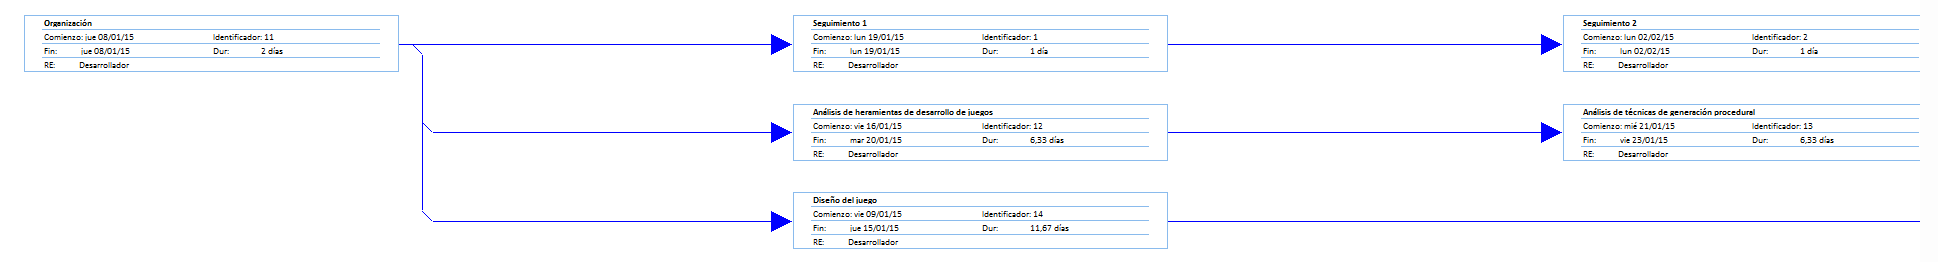
\includegraphics[scale=.4, angle=90]{fig/Red1}
	\caption{Diagrama de precedencias 1}
\end{figure}

\begin{figure}[!htbp]
	\centering
	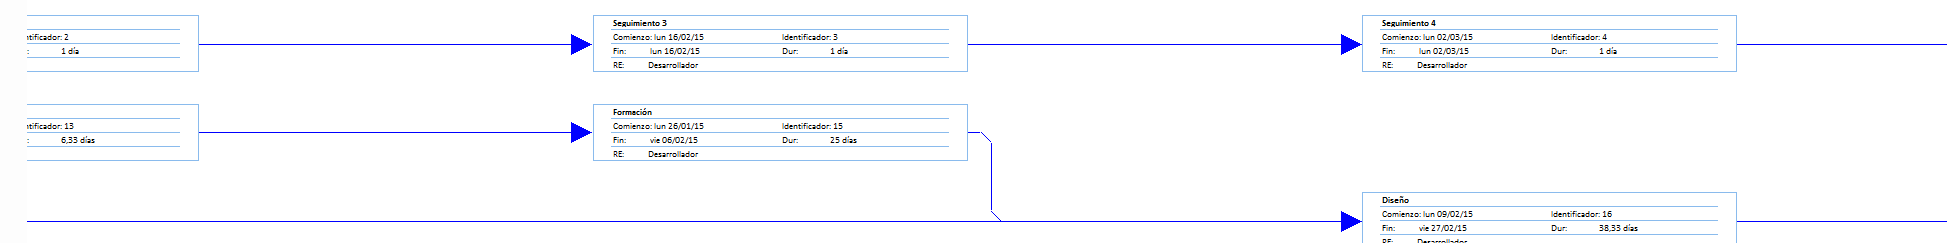
\includegraphics[scale=.4, angle=90]{fig/Red2}
	\caption{Diagrama de precedencias 2}
\end{figure}

\begin{figure}[!htbp]
	\centering
	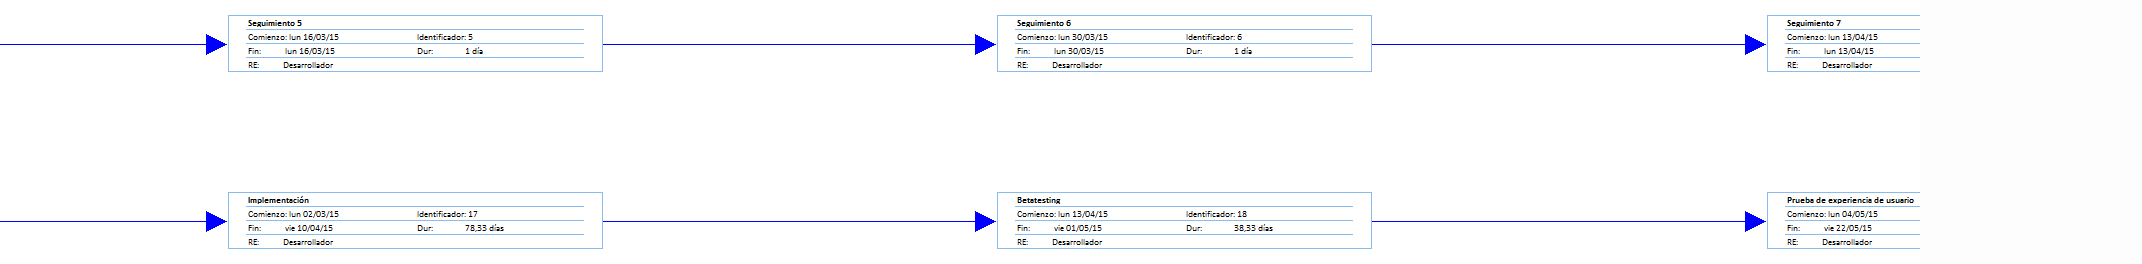
\includegraphics[scale=.4, angle=90]{fig/Red3}
	\caption{Diagrama de precedencias 3}
\end{figure}

\begin{figure}[!htbp]
	\centering
	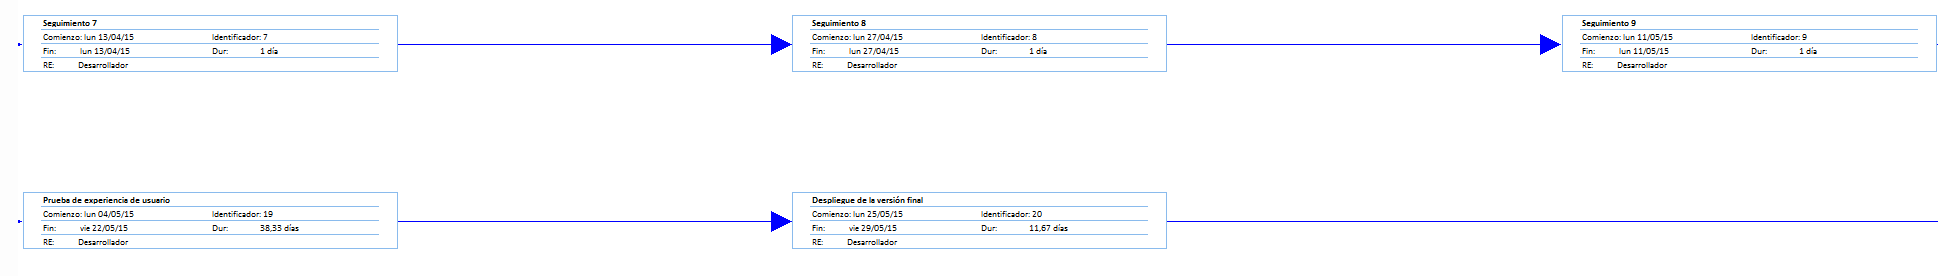
\includegraphics[scale=.4, angle=90]{fig/Red4}
	\caption{Diagrama de precedencias 4}
\end{figure}

\begin{figure}[!htbp]
	\centering
	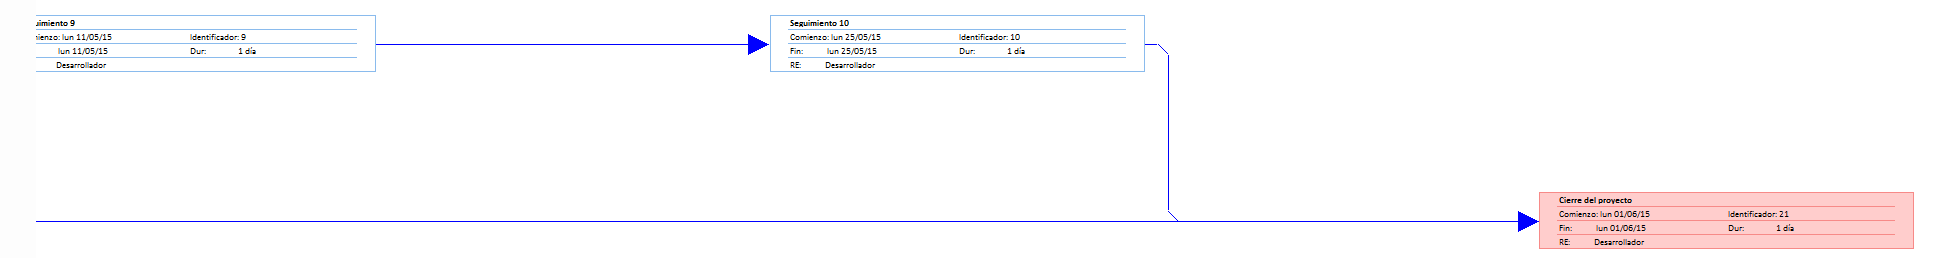
\includegraphics[scale=.4, angle=90]{fig/Red5}
	\caption{Diagrama de precedencias 5}
\end{figure}

\FloatBarrier

\section{Equipo Real}

El equipo real está formado por una única persona, que asumirá todos los roles del proyecto.

\begin{center}
	\captionof{table}{Carga de trabajo del equipo real}
	\begin{tabular}{|l|l|l|r|}
		\hline
		Nombre & Inicio & Fin & Trabajo(h) \\ \hline
		Desarrollador & 01/08/2015 & 1/06/2015 & 465 \\
		\hline
	\end{tabular}
\end{center}

\clearpage

\section{Plan de trabajo}

\begin{figure}[!htp]
	\centering
	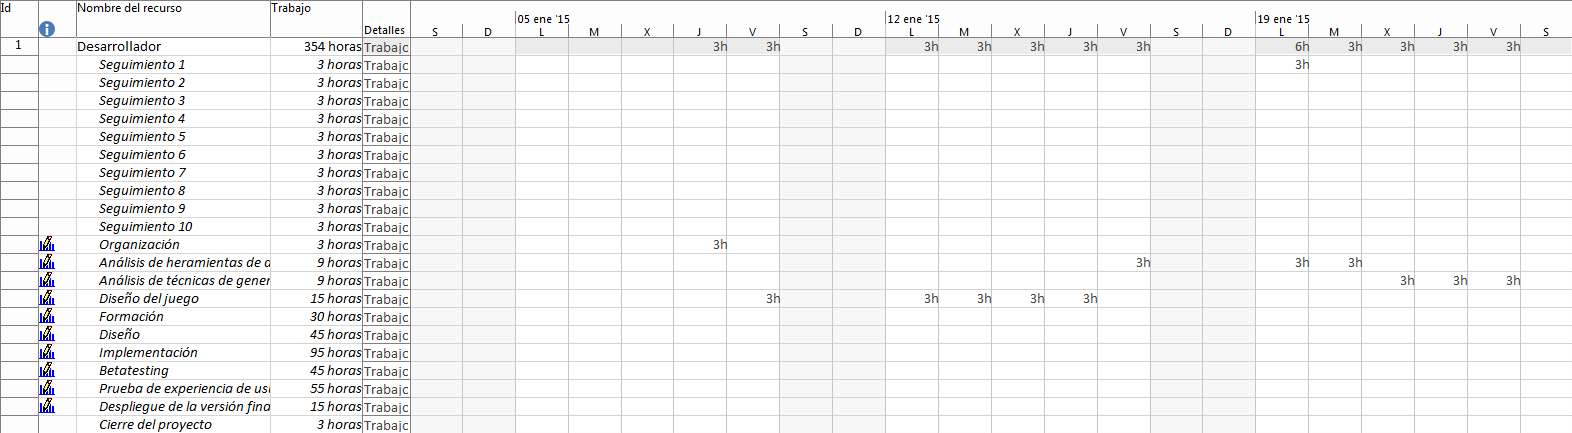
\includegraphics[page=1, scale=.5, angle=90]{fig/Plan1}
	\caption{Diagrama del plan de trabajo 1}
\end{figure}

\begin{figure}[!htp]
	\centering
	\includegraphics[page=2, scale=.5, angle=90]{fig/Plan2}
	\caption{Diagrama del plan de trabajo 2}
\end{figure}

\begin{figure}[!htp]
	\centering
	\includegraphics[page=3, scale=.5, angle=90]{fig/Plan3}
	\caption{Diagrama del plan de trabajo 3}
\end{figure}

\begin{figure}[!htp]
	\centering
	\includegraphics[page=4, scale=.5, angle=90]{fig/Plan4}
	\caption{Diagrama del plan de trabajo 4}
\end{figure}

\begin{figure}[!htp]
	\centering
	\includegraphics[page=5, scale=.5, angle=90]{fig/Plan5}
	\caption{Diagrama del plan de trabajo 5}
\end{figure}

\begin{figure}[!htp]
	\centering
	\includegraphics[page=6, scale=.5, angle=90]{fig/Plan6}
	\caption{Diagrama del plan de trabajo 6}
\end{figure}

\begin{figure}[!htp]
	\centering
	\includegraphics[page=7, scale=.5, angle=90]{fig/Plan7}
	\caption{Diagrama del plan de trabajo 7}
\end{figure}

\begin{figure}[!htp]
	\centering
	\includegraphics[page=8, scale=.5, angle=90]{fig/Plan8}
	\caption{Diagrama del plan de trabajo 8}
\end{figure}

\FloatBarrier

\section{Diagrama de Gantt}

\begin{figure}[!htp]
	\centering
	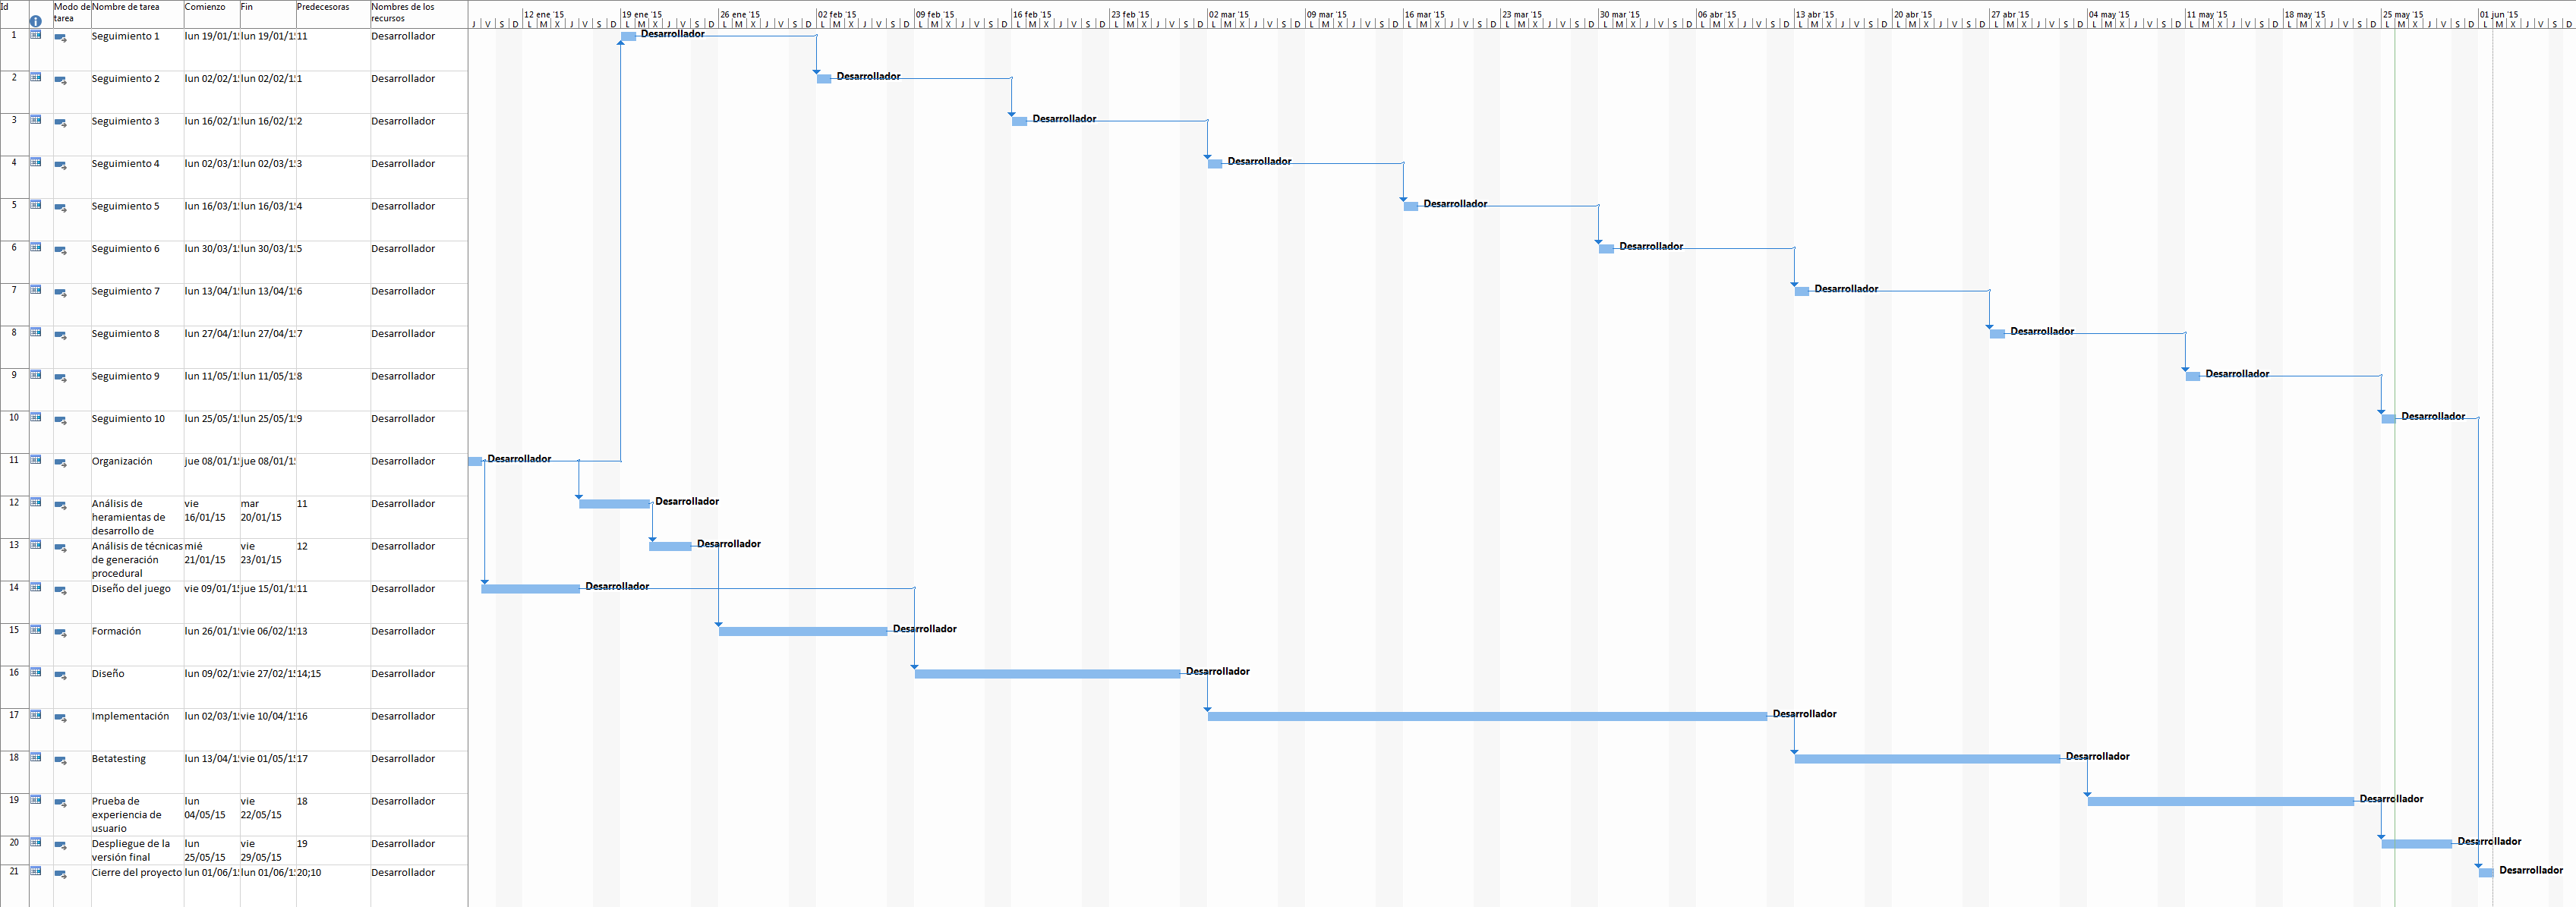
\includegraphics[page=1, scale=.25, angle=90]{fig/Gantt}
	\caption{Diagrama de Gantt}
\end{figure}

\FloatBarrier

\section{Estimación de cargas de trabajo por perfil}

\begin{center}
	\captionof{table}{Presupuesto: Cargas de trabajo por perfil}
	\begin{tabular}{|l|r|}
		\hline
		Perfil de trabajo & Carga de trabajo(h) \\ \hline
		Jefe de proyecto & 54 \\ \hline
		Programador & 321 \\ \hline
		Tester & 90 \\ \hline
		\hline
	\end{tabular}
\end{center}

\chapter{Presupuesto}

\section{Recursos Humanos}

\begin{center}
	\captionof{table}{Presupuesto: Recursos Humanos}
	\begin{tabular}{| l | r | r | r |}
		\hline
		Rol					&	Precio/hora(\euro/h)	&	Carga de trabajo(h)	&	Importe total(\euro)	\\	\hline
		Jefe de proyecto	& 	30						&	54 					& 	1620,00				\\	\hline
		Programador			&	25						&	321					&	8025,00			\\	\hline
		Tester			&	15						&	90					&	1350,00				\\	\hline
	\end{tabular}
\end{center}

\section{Recursos Software}

Como ya se ha dicho, todo el software utilizado para el proyecto será gratuito, de forma que no habrá gastos de este tipo.

\section{Recursos Hardware}

\begin{center}
	\captionof{table}{Presupuesto: Hardware}
	\begin{tabular}{| l | r | r | r |}
		\hline
		Nombre				&	Precio(\euro)	&	Unidades	&	Importe total(\euro)	\\	\hline
		Ordenador de sobremesa			& 	1500			&	1 			&	1500					\\	\hline
		Ordenador portátil	&	700				&	1			&	700						\\
		\hline
	\end{tabular}
\end{center}

\section{Total}

\begin{center}
	\captionof{table}{Presupuesto: Total}
	\begin{tabular}{| l | r |}
		\hline
		Tipo				&	Total			\\	\hline
		Recursos Humanos	& 	10995		\\	\hline
		Recursos Hardware	&	2200		\\	\hline
		\textbf{Total}		&	\textbf{13195}	\\
		\hline
	\end{tabular}
\end{center}